\documentclass[letterpaper, 10 pt, conference]{ieeeconf}  % Comment this line out if you need a4paper

%\documentclass[a4paper, 10pt, conference]{ieeeconf} % Use this line for a4 paper

\IEEEoverridecommandlockouts % This command is only needed if you want to use the \thanks command

\overrideIEEEmargins % Needed to meet printer requirements

\usepackage{cite}
\usepackage[pdftex]{graphicx}
\usepackage{multirow}
\usepackage[utf8]{inputenc}
\usepackage{color}
%\usepackage[table,xcdraw]{xcolor}

\usepackage{hyperref}
\hypersetup{
    colorlinks=true,
    linkcolor=black, % color of internal links
    citecolor=black, % color of links to bibliography
    filecolor=black, % color of file links
    urlcolor=black,
}

\title{\LARGE \bf On the use of vehicle categorization and context information for messages forwarding in VANETs}

\author{João B. Ribeiro$^{1}$, Wellington D. Branquinho Junior$^{1}$, Kifayat Ullah$^{1}$ and Edson dos Santos Moreira$^{1}$
%\thanks{*This work was supported by \textcolor{green}{National Council for the Improvement of Higher Education} (CAPES)}
\thanks{$^{1}$João B. Ribeiro, Wellington D. Branquinho Junior, Kifayat Ullah and Edson dos Santos Moreira are with Instituto de Ciências Matemáticas e de Computação (ICMC), University of São Paulo (USP), São Carlos, Brazil
    \tt\small \{joao.b, wellingtonjr\}@usp.br and \{kifayat, edson\}@icmc.usp.br}
}

%\thanks{$^{2}$Bernard D. Researchers with the Department of Electrical Engineering, Wright State University,
%        Dayton, OH 45435, USA
%        {\tt\small b.d.researcher@ieee.org}}%
%}

\begin{document}

\maketitle
\thispagestyle{empty}
\pagestyle{empty}

\begin{abstract}

With the increasing number of vehicles on the roads, traffic related problems like congestion, traffic jams, environmental pollution, and accidents, are very common these days. To solve transportation-related problems and make the driving experience safer, comfortable and enjoyable, VANETs were developed. A large number of applications ranges from safety to non-safety purposes are envisioned for VANETs. These applications make use of opportunistic encounters to forward messages. However, the unique characteristics of VANETs, make the opportunistic forwarding a challenging task. In this paper, we proposed a novel protocol called Message Forwarding by Categorization of Vehicles (\emph{MFCV}). Our protocol exploits contextual information and vehicles categorization to improve opportunistic forwarding of messages. We validate and compare our protocol with the Epidemic routing protocol, by means of a series of simulation experiments. Our protocol performed very close to the Epidemic protocol, in terms of messages delivery. Additionally, our results showed improved performance when vehicles categorization was considered in the forwarding decision. Finally, (\emph{MFCV}) performed better in terms of message latency, and resource utilization.

\end{abstract}

\IEEEpeerreviewmaketitle

\section{INTRODUCTION}

Vehicular Ad hoc NETworks (VANETs) are a subclass of Mobile Ad hoc NETworks with unique characteristics like high speed of nodes and dynamic network topology. To disseminate data, VANETs enable communications between mobile nodes and infrastructure network. These networks support a large number of applications such as accident avoidance, intelligent traffic control, and data dissemination, thereby, providing safety, comfort, and convenience to the users \cite{conprova2013}.

The nodes (vehicles) in VANETs contain hundreds of onboard sensors, which provide useful information about vehicle state (e.g., engine status, vehicle position, speed, heading) and surrounding environment (e.g., road and traffic condition, and weather forecast). Vehicles that collect, disseminate and make use of this contextual information are called context-aware vehicles \cite{grilli2009}. Context-awareness is important for the deployment of a large number of new applications. However, providing reliable and efficient dissemination of contextual information is a challenging task in VANETs. It is important to share only relevant information among vehicles, in order to reduce the communication overhead \cite{kumar2015}.

The importance of vehicles categorization for providing contextual information has been recently addressed in \cite{zhang2012, zhang2014}. We can categorize the vehicles into a taxi, bus, private car, and cargo. Each of them has a different mobility pattern. For example, a bus has its own predefined route, timing, and schedule. On the other hand, a taxi has no restricted mobility and it can follow different routes at different times, based on passengers demands and drivers preferences. Such mobility information could be used to select an appropriate node for carrying a message towards its destination.

Ontologies could be used to ensure interoperability among VANETs applications. It also facilitates the process of sharing and using contextual information \cite{madkour2011}. Additionally, ontologies could help to represent the different categories of vehicles, how they relate with each other and with the context data. Furthermore, it assists in messages forwarding process.

Motivated by the works presented in \cite{Yokoyama_2014, ullahadvertising} that make use of beacon messages and opportunistic vehicles communications to exchange information, we propose Message Forwarding by Categorization of Vehicles (\emph{MFCV}). \emph{MFCV} is an opportunistic message forwarding protocol that makes use of beacons and exploits contextual information, especially the vehicle usage category, to improve the messages delivery by consuming relatively low resources.

We consider a scenario where vehicles create messages to be forwarded for a globally known fixed infrastructure. However, to deliver these messages, intelligent forwarding decisions are required. In this regard, our protocol uses three different schemes, i.e., vehicle distance to the destination, vehicle speed, and its category. Additionally, we used a mechanism called \emph{RateTimeToSend} which uses traffic flow information to control message forwarding rate. To evaluate the performance of our protocol, we performed an extensive set of simulations by considering different parameters.

This rest of this paper is organized as follows. Section II reviews the related works about context-awareness and ontologies for VANETs. Section III gives an overview of contextual information and its use in opportunistic forwarding. Section IV discusses the use of ontologies for categorization of vehicles. Section V presents our proposed protocol. Section VI presents simulation results and performance evaluation of our protocol. Finally, Section VII concludes this paper with some future directions.

\section{RELATED WORKS}

In \cite{magf2009}, the authors addressed the problem of rapid topology changes and frequent disconnections in VANETs. They assumed that the vehicle is aware of its own movement and its neighbors, and uses this information to select the best next hop to carry the message. They concluded that using a combination of position, speed and direction have a significant performance improvement in terms of data delivery ratio and latency.

A geocast forwarding protocol for VANETs was proposed in \cite{vcarp2012}. The protocol uses context information in order to make a more accurate decision in the forwarding process. Besides, it used a shared cache mechanism to prevent packet losses, due to full caches. Using shared cache mechanism along with position, distance to destination and direction, they achieved an improvement of 40\%, in terms of packet delivery ratio. Additionally, they reduced the overhead to 89\%, as compared with \cite{maihofer2004}.

In \cite{move2005} five opportunistic forwarding schemes were presented and compared in terms of overhead, success rate, and latency. In the first scheme, the vehicle gets the message and carries it towards the destination, without exchanging data with other nodes. Whereas in the second scheme, the message is broadcasted to all nodes, moving towards the destination. In the remaining schemes, they used the context related information, i.e., distance, speed, and heading.

In order to better utilize node mobility and deal with connectivity issues, \emph{GeoMob} \cite{zhang2014} was proposed. The scheme exploits the different mobility patterns of the two categories of vehicles, taxicabs and buses. Furthermore, a global traffic distribution was used to create cluster regions and forward the message through them. However, they used dynamic clusters which generate overhead. Moreover, their solution requires the global traffic distribution which may not be available. These requirements could degrade performance or even make the solution impracticable.

A lightweight vehicular ontology was proposed in CAOVA \cite{caova2012}, with the aim to share and reuse information about accidents. Based on the ontology, they generate warnings to improve the safety on the roads. Similarly, \cite{groza2014} proposed a vehicular network ontology to facilitate the interoperability at the application level. They showed the capabilities of ontologies to enhance the information collection, representation and its use for preventing accidents.

The aforementioned studies partially address the use of contextual information, e.g., position, speed and categorization of vehicles in order to improve the opportunistic forwarding of messages and ontologies to ensure interoperability among them. We intend to combine the ideas of these approaches in order to improve the opportunistic forwarding of messages, focusing on vehicles categories and \emph{RateTimeToSend} mechanism.

\section{VEHICLES AND ENVIRONMENT CONTEXTUAL INFORMATION}

Dey \cite{dey2001} defines context as “any information that can be used to characterize the situation of an entity. An entity is a person, place, or an object that is considered relevant to the interaction between a user and an application, including the user and applications themselves.” A system that makes use of this sort of information is called context-aware system. Such systems achieve improvements in the quality of information and providing better services to the user. Context-aware systems are adaptable to  different situations, or context, without user intervention \cite{baldauf2007}.

By utilization the embedded sensors, a smart vehicle can produce rich context information. The context information about vehicle contains speed, direction, wheel friction, acceleration and position of the vehicle. Furthermore, a smart car would monitor its environment. The context information about the environment can be divided into static (e.g., road signs, number of lanes), and dynamic (e.g., wind speed, range of visibility, chances of rain). Using context information of the vehicle or environment make it possible to detect or prevent hazardous situations. Moreover, the context can also be useful in the knowledge distribution over a vehicular network \cite{tocadas2010}.

An example of a network that could make use of context information are the opportunistic networks, which take advantage of opportunistic encounters (not scheduled) to exchange data and share contextual information  \cite{geoopp2014}. Being aware of its neighbors and message destination position, a node can forward incoming messages towards the destination, by selecting the node that is geographically closer to the destination \cite{gpsr2000}. This way, the message could be forwarded accurately by using information about immediate neighbors only \cite{magf2009}.

The \autoref{context} shows some context information, regarding the \emph{driver}, the \emph{environment} and the \emph{vehicles}. This context information can be use to improve VANETs applications, such as advertising and entertainment. Some possible use cases are a) sending warning message to the neighborhood about a reckless and fatigued driver; b) disseminating context-aware services advertisements to the nearby drivers; c) alerting drivers about traffic density and road conditions.

\begin{table}[ht]
    \center
    %\renewcommand{\arraystretch}{1.2}
    \caption{Context information subset} \label{context}
    \begin{tabular}{|c|l|l|}
        \hline
        Entity & \multicolumn{1}{c|}{Feature} & \multicolumn{1}{c|}{Value} \\ \hline
        \multirow{4}{*}{Driver} & Age & under\_18; 18-65; 65+ \\ \cline{2-3}
        & Behavior & prudent, reckless \\ \cline{2-3}
        & Condition& drunk, fatigued, normal \\ \cline{2-3}
        & Mood & anxious, calm, stressed \\ \hline
        \multirow{5}{*}{Environment} & Road Conditions& dry, flooded, snow, wet \\ \cline{2-3}
        & Road Type& dual carriage way, one way \\ \cline{2-3}
        & Traffic Density& low, medium, high \\ \cline{2-3}
        & Time & out\_peak\_time, peak\_time \\ \cline{2-3}
        & Weather Condition& fog, raining, snowing \\ \hline
        \multirow{5}{*}{Vehicle} & Category & bus, cargo, private car, taxi \\ \cline{2-3}
        & Condition& brake, engine, headlights \\ \cline{2-3}
        & Movement & acceleration, heading, speed \\ \cline{2-3}
        & Size & length, width, height, mass \\ \cline{2-3}
        & Trip & contacts, path history, position \\ \hline
    \end{tabular}
\end{table}

\section{USING ONTOLOGY FOR VEHICLES CATEGORIZATION}

In this section, we explain the use of ontologies for vehicles categorization.

Ontology is an organized form of representing the data. It is used to represent different kinds of objects and show the relationship among them. It provides a common vocabulary to enable interoperability, resolve ambiguity and hence to describe concepts and the relations that exist between them \cite{madkour2011}.

A single ontology for an area is not sufficient, as it can grow fast and will require increasing amount of resources to host, manage, and use. Hence, there is a need for more than one ontology. In the case of more than one ontology, they are classified according to the level of detailed knowledge they provide \cite{packer2010}. Consequently, we have more than one ontologies for the vehicular scenarios (e.g., for sales, used cars, manufacture).

Ontology for context information can be use as a formal context model that allows an efficient gathering, managing and storing the context information. Likewise, it provides interoperability in heterogeneous systems, by defining a common set of concepts about context while interacting. It also enables reasoning mechanisms to infer high-level information from a raw context, find and solve inconsistencies. Additionally, it facilitates the reuse of the knowledge \cite{serrano2007}.

For our work, we used the ontology\footnote{Draft available on (http://auto.sdo-gao.appspot.com/) Access in: 14 June 2016} proposed in \cite{gao_2016} that categorizes the vehicle according to its physical features (e.g., size of the vehicle, the number of axes) to represent the vehicles categories. Furthermore, we also need to categorize the vehicles by its usage (i.e., private car, taxi). Therefore, we have added in the ``\emph{CarUsageType}'' a vehicle usage category. This category defines how the vehicle will be used and allows the extraction of mobility patterns information. The physical category should be used by traffic management companies, for instance, in the toll collection. While, the usage category can be used by forwarding protocols to decide which node is the best to carry a message. In our protocol, the vehicle usage category information is sent by vehicles, along with other information collected from sensors.

\section{Message Forwarding by Categorization of Vehicles}

Performing real world experiments, to test and evaluate VANETs applications is very costly and laborious. An alternative approach is to use simulators. We performed simulations to validate our protocol called \emph{MFCV}. We used Simulation of Urban Mobility (\emph{SUMO}) \cite{SUMO-2012} to create the mobility model, including the environment and the vehicles routes. To specify the number of vehicles, their positions, speed and acceleration we modified the configurations files of the simulation manually. To simulate the communication between the vehicles and infrastructure, we used the framework \emph{Veins} \cite{veins2016} on top of \emph{OMNeT++} simulator \cite{omnet2016}. The parameters used for our experiments are given in the \autoref{simulation-param}.

\begin{table}[ht]
    \center
    %\renewcommand{\arraystretch}{1.2}
    \caption{Simulation Parameters} \label{simulation-param}
    \begin{tabular}{|c|c|}
        \hline
        Packet format                  & WAVE short message \\ \hline
        Status beacon Interval         & 1 second           \\ \hline
        Validity of status beacons     & 3 seconds          \\ \hline
        Message creation interval      & 15 seconds         \\ \hline
        Beacon Length                  & 512 KB             \\ \hline
        Destination Position           & (1500, 1500)       \\ \hline
        Transmission ranges of vehicles & 250 meters         \\ \hline
        Simulation time                & 600 seconds        \\ \hline
        Maximum number of hops         & 10 hops            \\ \hline
    \end{tabular}
\end{table}

In \emph{MFCV} we assume that each vehicle is able to collect the required contextual information about itself and store information received from its neighbors. Furthermore, the contextual information shared among the vehicles is reliable and the vehicles collaborate with the forwarding process since security is not the focus of this work. In the following subsections, we define the models used for the implementation.

\subsection{Propagation Model}

For network and transport layers, we used WAVE Short Message Protocol (WSMP) standard. We have adopted the IEEE 802.11p standard protocol for the PHY and MAC layers. For multichannel operation, we used the IEEE 1609.4 standard protocol. The signal propagation was made according to the Simplified Path-Loss model, described in \cite{tse2005}.

\subsection{Mobility Model}

We developed a mobility scenario that consists of a grid of 9 km$^2$ (urban area) using the \emph{netgenerate} tool from SUMO. In order to evaluate the influence of the different categories of vehicles in the forwarding decision, 10 vehicles were classified as taxis and the remaining as private vehicles. We used \emph{randomTrips}, SUMO for generating routes, in which the taxis accomplished 15 km while the private vehicles only 2 km. Due to this, the taxi will take maximum simulation time (i.e., 10 minutes) to complete its route, whereas the private vehicles leave the scenario in approximately 2 minutes. This way, the taxis can increase the successful delivery rate of messages as compared to private vehicles.

Initially, 10 taxi and 40 private vehicles enter in the scenario. After 2 minutes, additional 40 private vehicles enter in the scenario. After an interval of 2 minutes, 40 new private vehicles enter the scenario. This ensures that at any time the ratio of private vehicles to taxis will be 4 to 1. A total of 210 vehicles (200 private vehicles and 10 taxis) participate in the experiment.

\subsection{Network Model}

The \emph{MFCV} consist of two different phases, Discovery and Forwarding, wherein the vehicles collect data from its neighbors and used the information to make forwarding decisions, respectively.

\subsubsection{Discovery Phase}

The first phase of \emph{MFCV} is to discover the neighborhood of a vehicle and creates a \emph{neighbors' table} (hash table). The table contains information about the neighbors' ID, its current and a previous geographical position (5 seconds ago), categories (type and use), speed and a timestamp. Each vehicle broadcasts this information, with an interval of 1 second, in a message called \emph{status beacon}. When a vehicle receives a \emph{status beacon}, it can either store it as a new entry in the table or update an entry, if it already exists. This information remains valid for 3 seconds in the vehicle buffer. This information helps the vehicles to make more accurate decisions in the \emph{Forwarding Phase}.

\subsubsection{Forwarding Phase}

In the second phase, the messages are forwarded, using \emph{neighbors' table} information, to improve the forwarding decisions. Random vehicles are chosen to create the messages during the simulation. When a vehicle enters the scenario, it may create a new message and a schedule to try to send it according to its \emph{RateTimeToSend} value. The content of this message contains 4 IDs (i.e, source, temporarySender, temporaryReceiver, and destination), the hopCount (number of hops to reach the destination), the TTL, the message by itself and timestamp. The vehicle will try to send the message to the neighbor with the best probability, based on the information in the neighbors' table, to deliver the message. If the destination is one of the neighbors, the message is delivery to it. The message has a maximum allowed time (TTL - Time To Live) in the simulation. The value of TTL is 60 or 120 seconds. Once the TTL is expired, the message is discarded from the buffer. Moreover, if a node receives a message and its buffer is full then the oldest message is discarded.

The decision-making process was divided into three different schemes. In the first scheme, the node with the shortest distance to the destination was chosen to carry the message. The distance and speed of the nodes were used in the second approach. In the third scheme, another information was exploited, i.e., the categories \emph{taxi} and \emph{private vehicles} and its respective mobility patterns. In all experiment, we used a path history of each vehicle, that contains its current and 5 seconds old position, as a way to know if the vehicle is moving towards the destination, hence being a good option to carry the message.

Due to wide and flexible mobility, the \emph{taxi} has a higher chance to deliver the message successfully as compared to the \emph{private vehicles}. To prevent the \emph{taxis} to be overloaded, \emph{taxis} had a 80\% chance of selection, in the decision process. Additionally, we developed a mechanism called \emph{RateTimeToSend} that is a value, linked with the vehicle speed, it ensures that vehicles with low speed (under 10 m/s) do not flood the network. In the case of traffic jams it controls a number of messages forwarded.

Initially, its value is 2.5 seconds for all vehicles. After 2.5 seconds the vehicle tries to forward the first message in the buffer, and schedule to forward the next message in 2.4 or 2.6 seconds according to its mobility. The value increases 0.1 seconds if the vehicle does not move 10 meters in 1 second, otherwise, the value decreases 0.1 s. The value is always between 0.1 and 5 seconds. When the vehicle run its whole vector it will check if have passed 5 seconds since it sends the first message, if so, it will start to send the messages from the beginning of the buffer (just as before), if it is not the case it will wait for 5 seconds to start from the beginning.

\subsection{Scenario}

In our simulation scenario, we installed a single Road-Side Unit (RSU), in the middle of the scenario. This RSU is the destination point of all messages. The vehicles (both private vehicles  and taxis), enters the scenario, at the point defined by its routes. We run the simulation for a total of 10 minutes. Furthermore, the buffer was capable of handling 50 messages at a time.

A total of 12 experiments were carried out, having 4 different combinations and 5 replications for each one. At each replication, different vehicles were selected to generate messages. However, same replications of different combinations generate the same traffic and messages. For example in the first experiment, the first replication selects the same vehicles as in the second replication of the second experiment.

Depending on the experiment, the number of vehicles that generate the message, every 15 seconds, can be either 1 or 2. To guarantee that the message would stay in the scenario its TTL (i.e., 60, 120 or 150s according to the experiment) the messages will be created until 450 seconds of simulation time. Hence, at the end of the simulation, a total of 30 or 60 messages are created.

\section{PERFORMANCE EVALUATION}

In order to validate our proposal we compared our results with \emph{Epidemic} Routing protocol \cite{Vahdat-2000}. In this approach, each vehicle has a message buffer where it stores received and created messages with a unique global ID and a \emph{summary vector}.

When two nodes are in communication range, the node with lower ID starts the \emph{anti-entropy session}. So it sends its \emph{summary vector} to the other node. After analyzing the vector the node generates a \emph{request messages vector} with their IDs. On receipt, the first node sends the requested messages, after that the opposite is done. Thus, both now have the union of their messages.

To avoid unnecessary message exchanges and resources usage, before each \emph{anti-entropy session}, it is observed if the nodes have not met in the last 7 seconds, which is approximately the time that they take to reach the middle of their communication range. We selected 10 as a maximum number of hops that a message can take until arrives at its destination. Additionally, we used 60, 120 or 150 seconds as the \emph{TTL} for the message, regarding of the experiment being executed.

To evaluate the success of \emph{MFCV}, we used three metrics: delivery success rate, message packets sent per minute and average latency. Firstly, we measure the percentage of packets that reached the destination. Secondly, we evaluate the number of packets generated to deliver the messages, including Epidemic operational messages. Finally, the average latency, measure the average time taken to deliver the messages. We used the abbreviations \textbf{\emph{D}} that stands for \textbf{D}istance, \textbf{\emph{DS}} for \textbf{D}istance and \textbf{S}peed, and textbf{\emph{DSC}} for \textbf{D}istance, \textbf{S}peed and \textbf{C}ategory to represent the information exploited in each scheme.

\subsection{Delivery success rate}

In the first experiment, we compared \emph{MFCV}, exploiting different context information, with the \emph{Epidemic} protocol measuring the number of messages that reached the destination. Since \emph{Epidemic} is a sort of controlled flooding, its successful delivery rate is very high, so our goal was to reach closer to its results.

In this experiment, a vehicle was chosen to create a message every 15 seconds, for delivery, generating a total of 30 messages. 
As seen in \autoref{grafico1} the combination \emph{DSC} (distance, speed, and category) shows an improvement of approximately 6\% when compared to the basic D (distance) and is 9\% below the performance of \emph{Epidemic}. Increasing the number of generated message to 60 with the TTL equal to 60 seconds, we get same results for \emph{D}, \emph{DS} and \emph{DSC}, but 6\% below the \emph{Epidemic} performance. Increasing the TTL to 120 seconds, the results of \emph{DSC} shows 5\% better performance than \emph{D} and \emph{DS}, but 12\% below \emph{Epidemic}. We compared both \emph{Epidemic} and \emph{DSC}, with 60 generated messages, increasing message TTL to 150 seconds, and the results displayed in \autoref{grafico2} show 100\% delivery success rate to \emph{Epidemic} and 98\% to our approach.

\begin{figure}[thpb]
    \center
    \framebox{
        \parbox{2.1in}{
            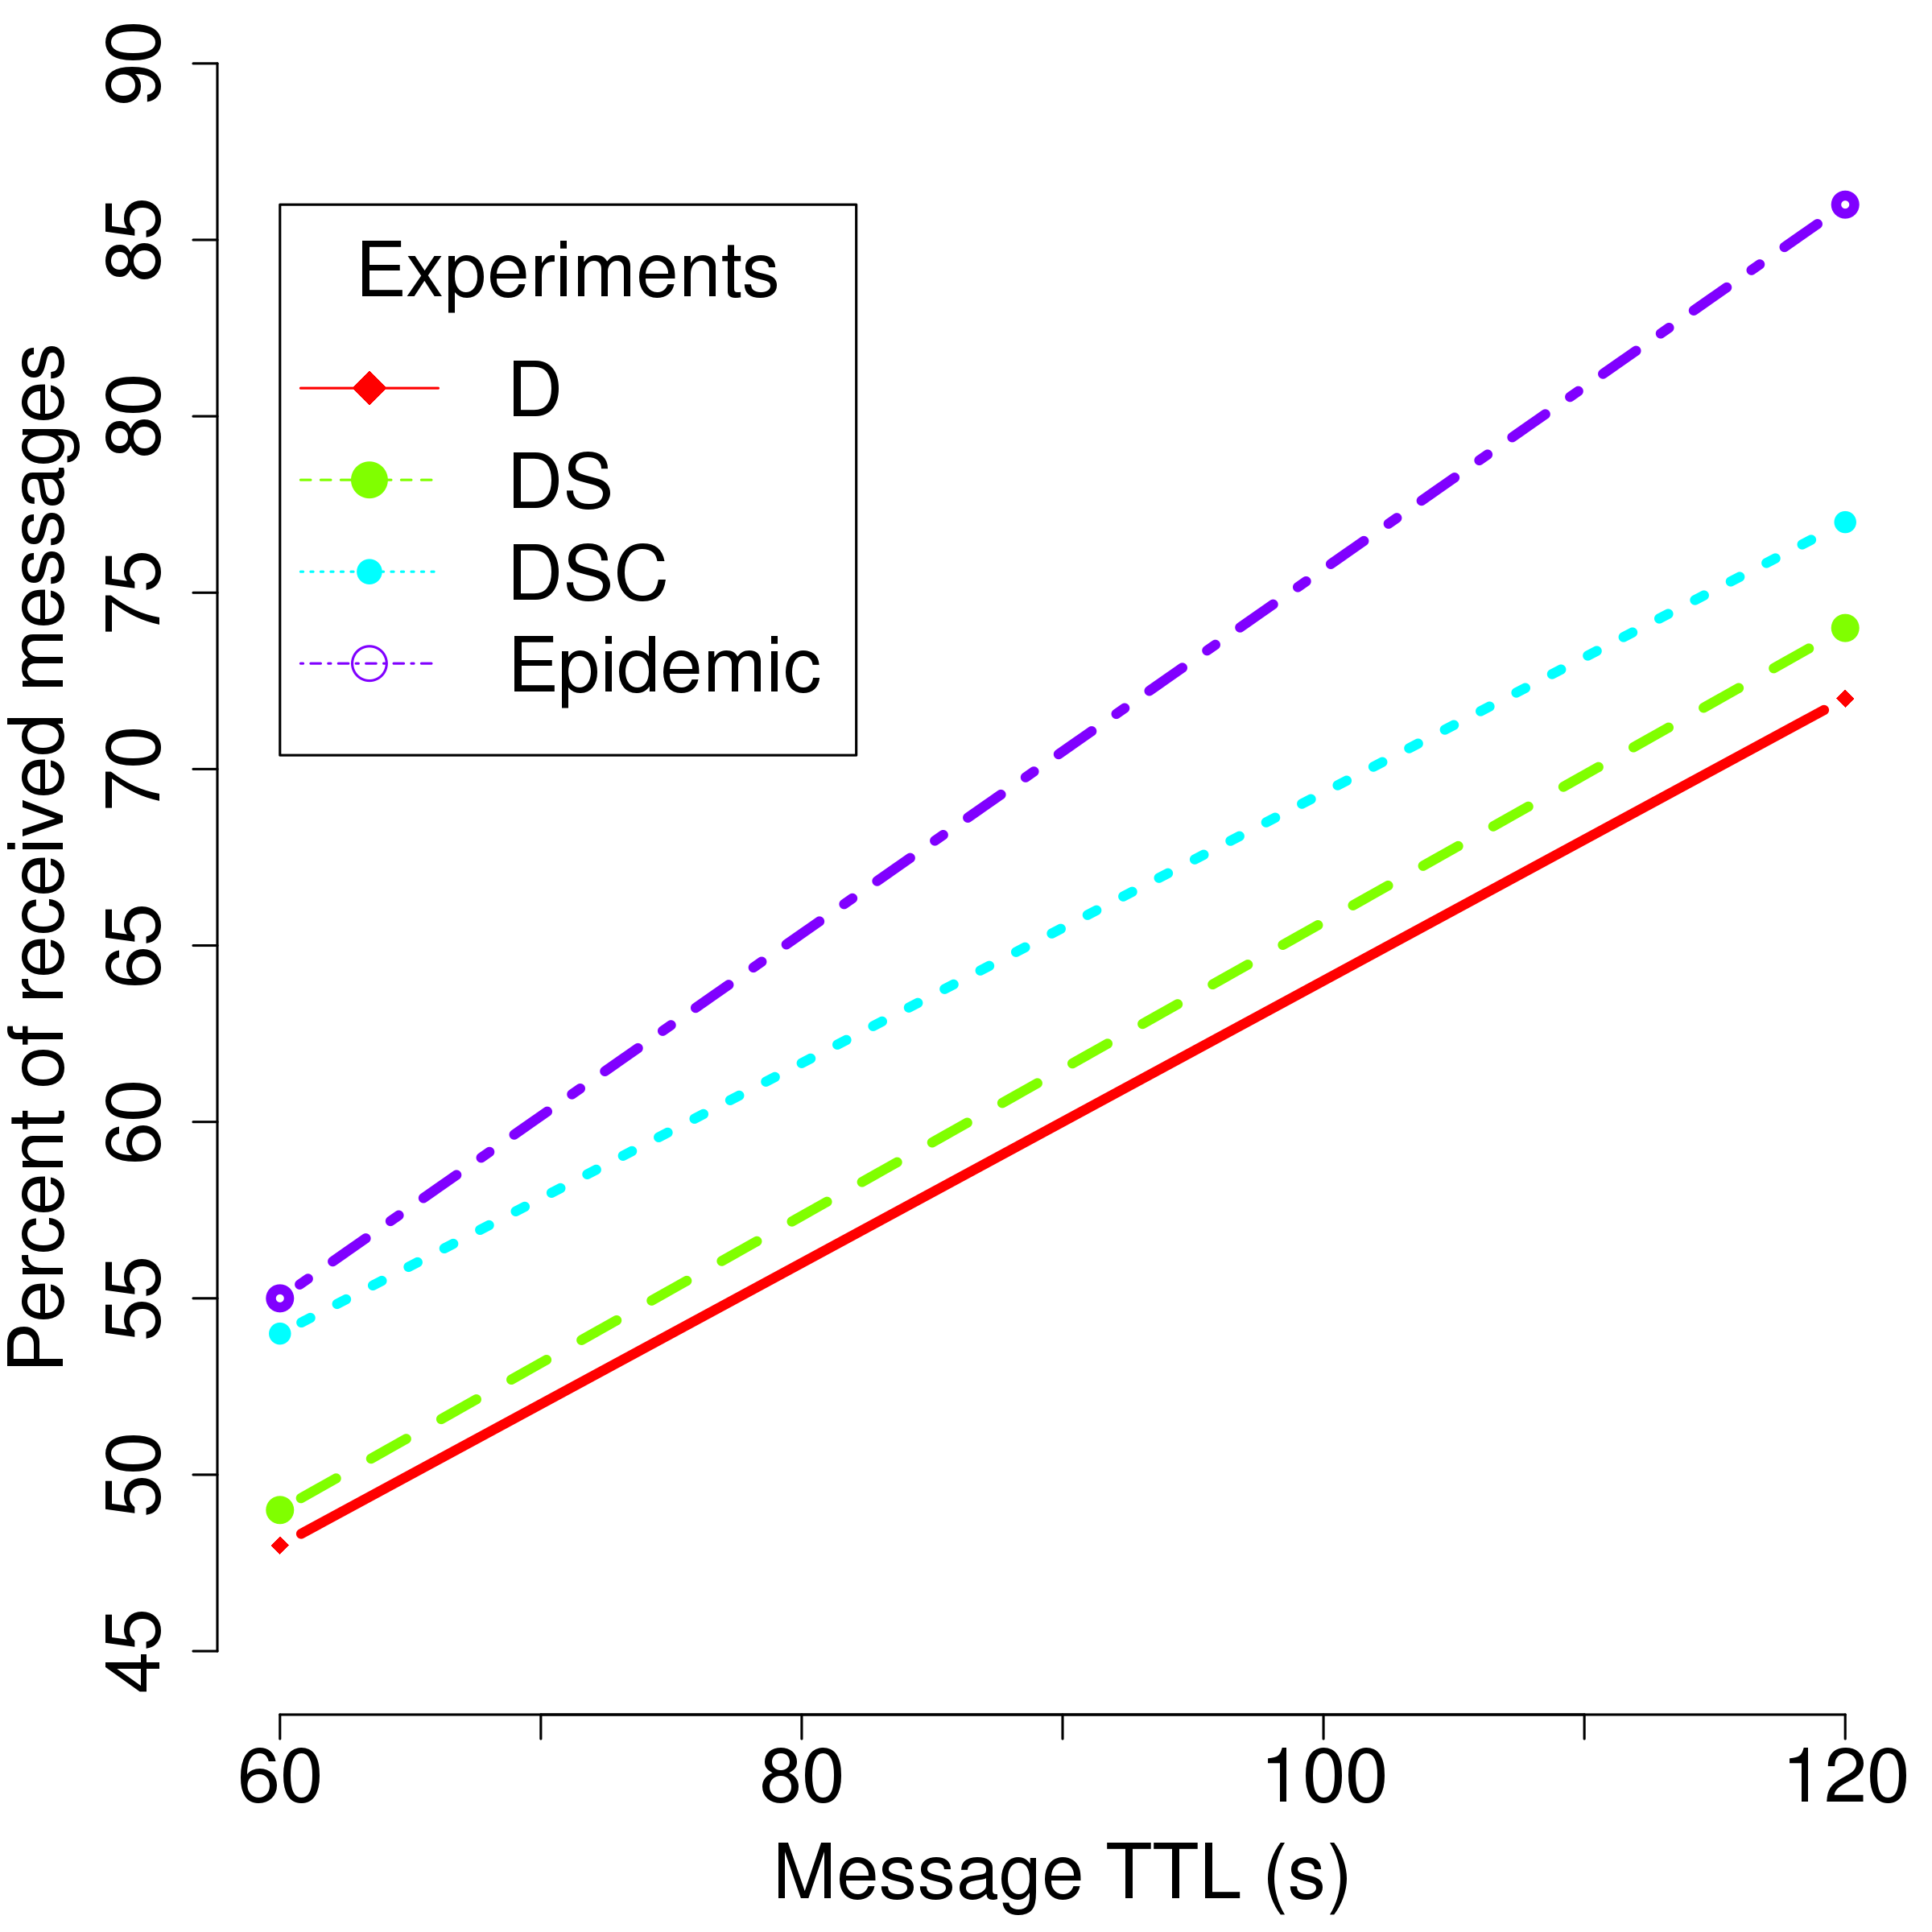
\includegraphics[width=5.3cm]{img/1.png}
        }
    }
    \caption{Percentage of messages delivered in function of the message TTL with 30 messages} \label{grafico1}
\end{figure}

\begin{figure}[thpb]
    \center
    \framebox{
        \parbox{2.1in}{
            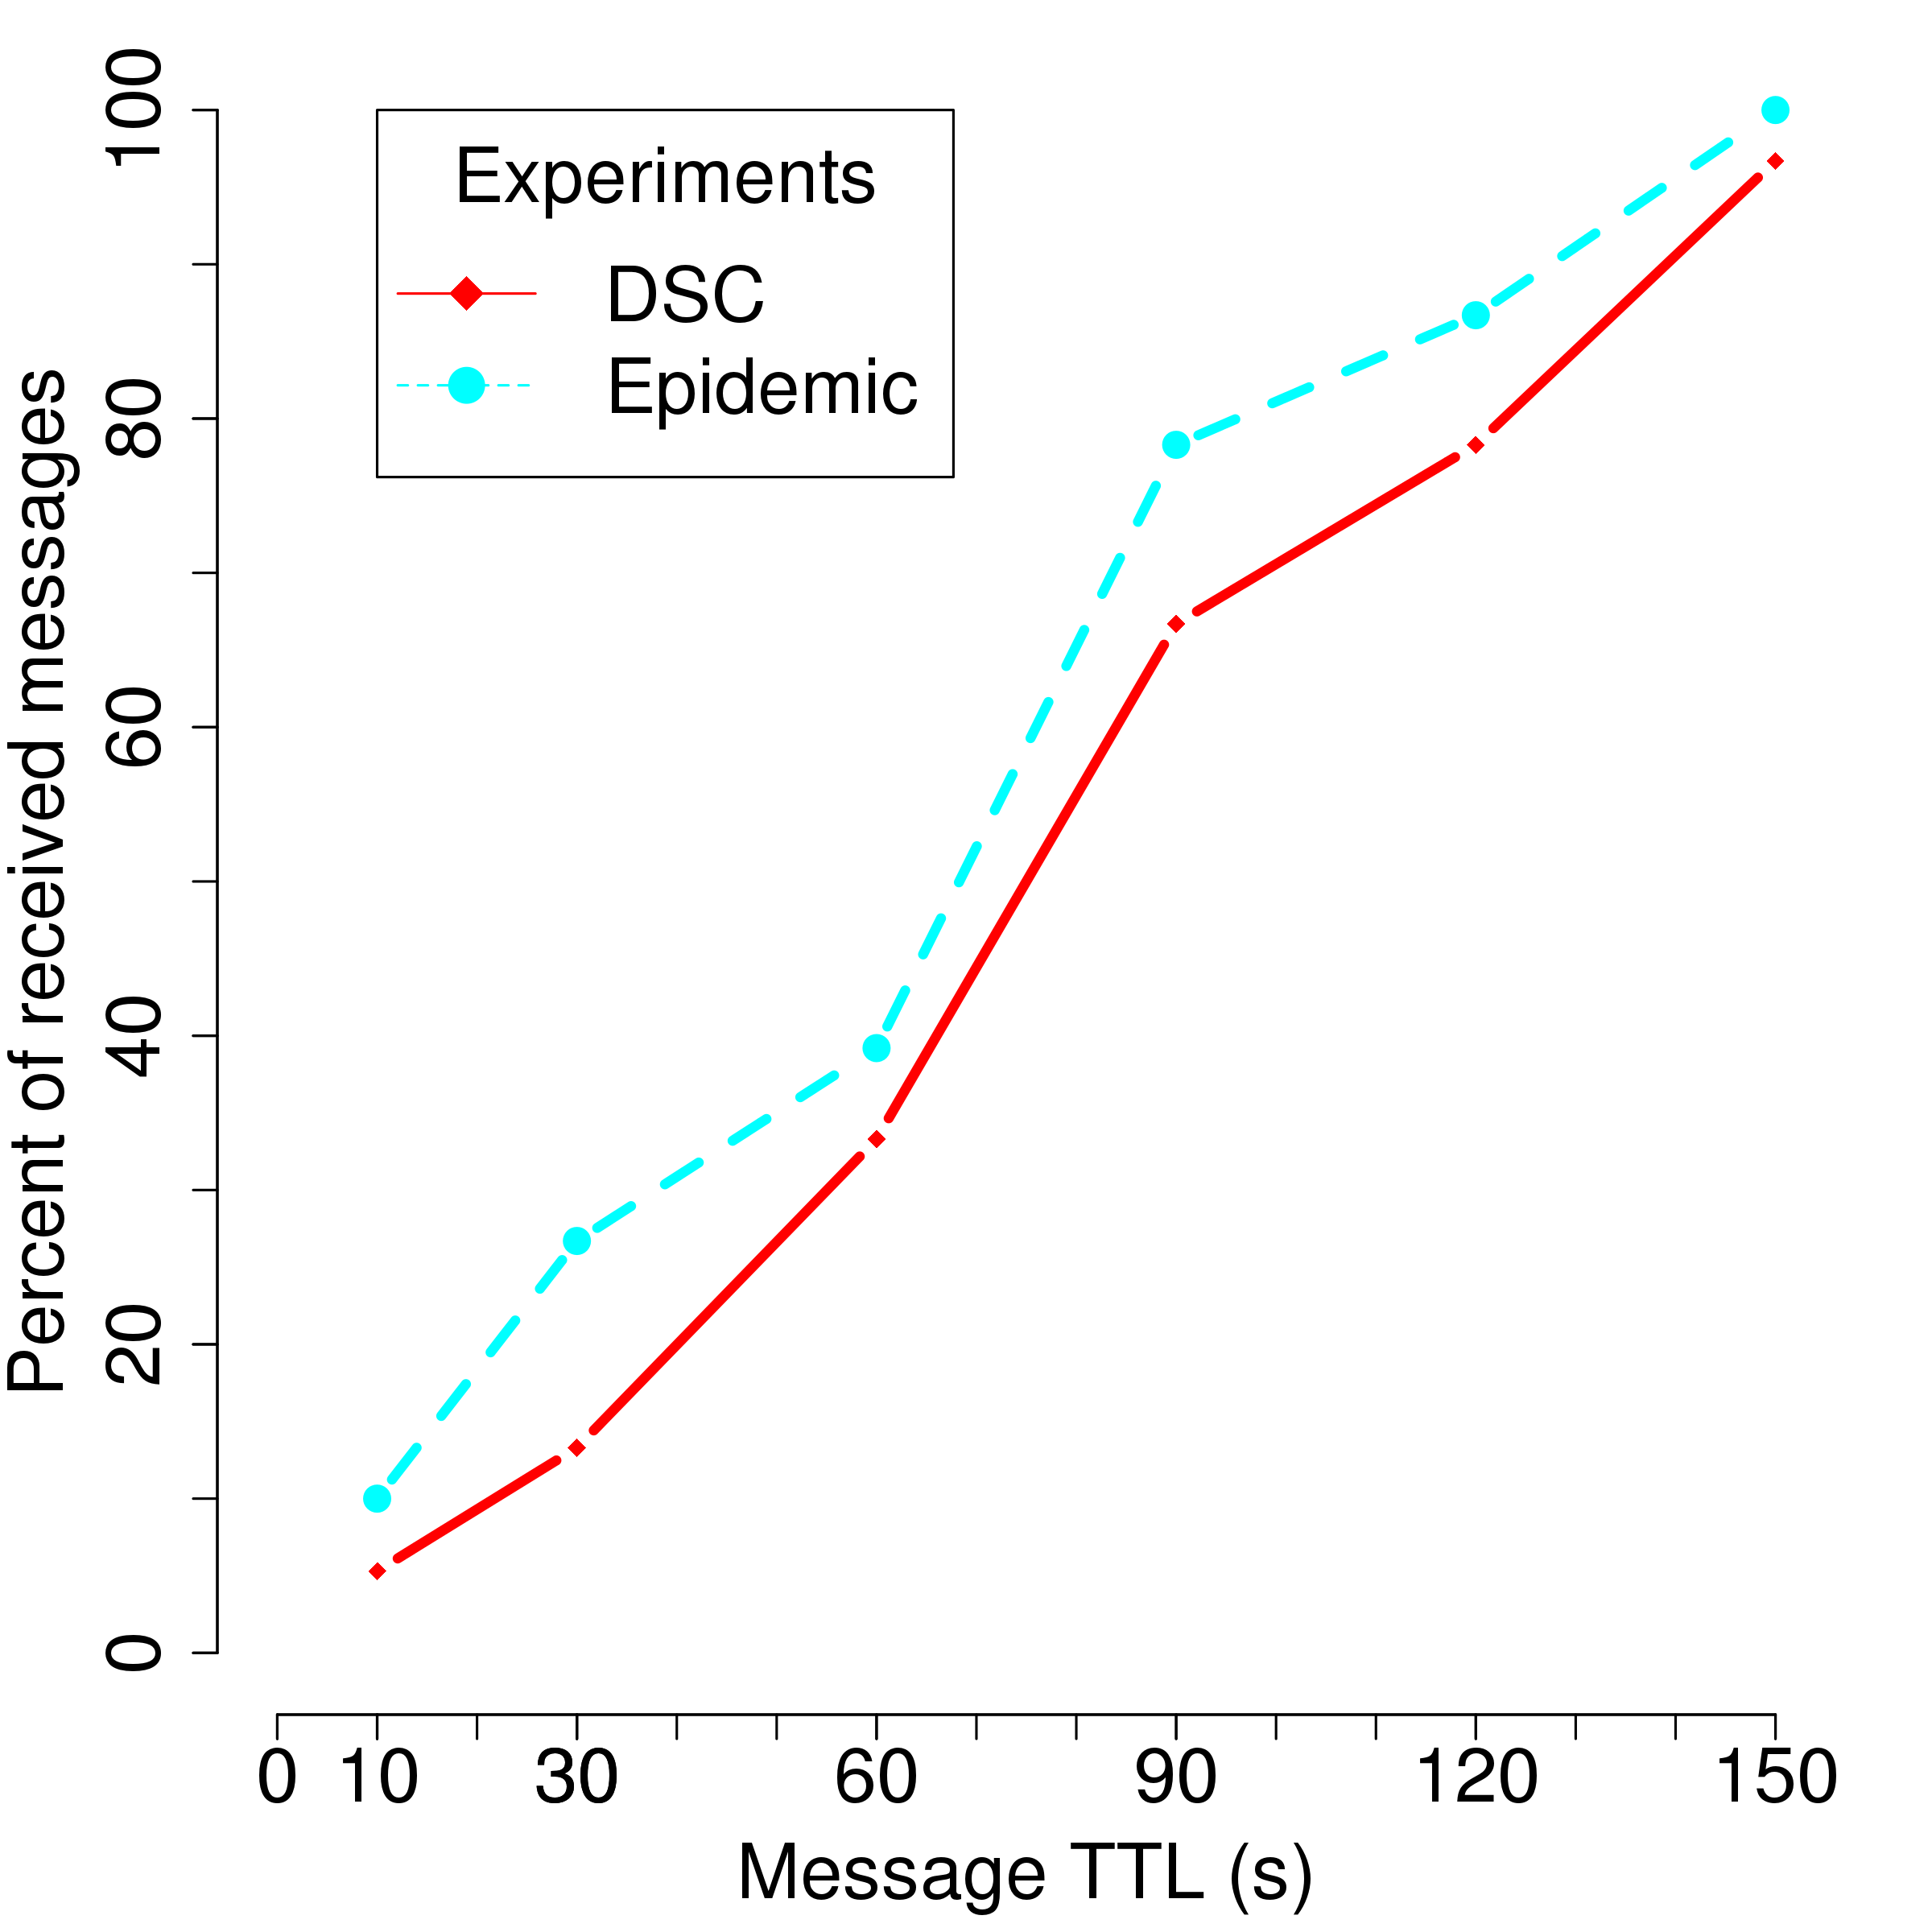
\includegraphics[width=5.3cm]{img/7.png}
        }
    }
    \caption{Percentage of messages delivered in function of the message TTL with 60 messages} \label{grafico2}
\end{figure}

\subsection{Average latency}

This metric evaluated the average time that the messages have spent to reach the destination. The \autoref{grafico3} shows that the same results to D and DS and a very similar to DSC, but when compared to Epidemic the DSC had a latency 10\% lower when the message TTL was 60 and 16\% when it was 120. This is due to the fact that our proposal chose the node that is closest to the destination, moving towards it and is moving faster. Moreover, the category helps us to select the nodes that have a higher chance to met the destination according to its mobility patterns instead of doing a controlled broadcast it like Epidemic does.

\begin{figure}[thpb]
    \center
    \framebox{
        \parbox{2.1in}{
            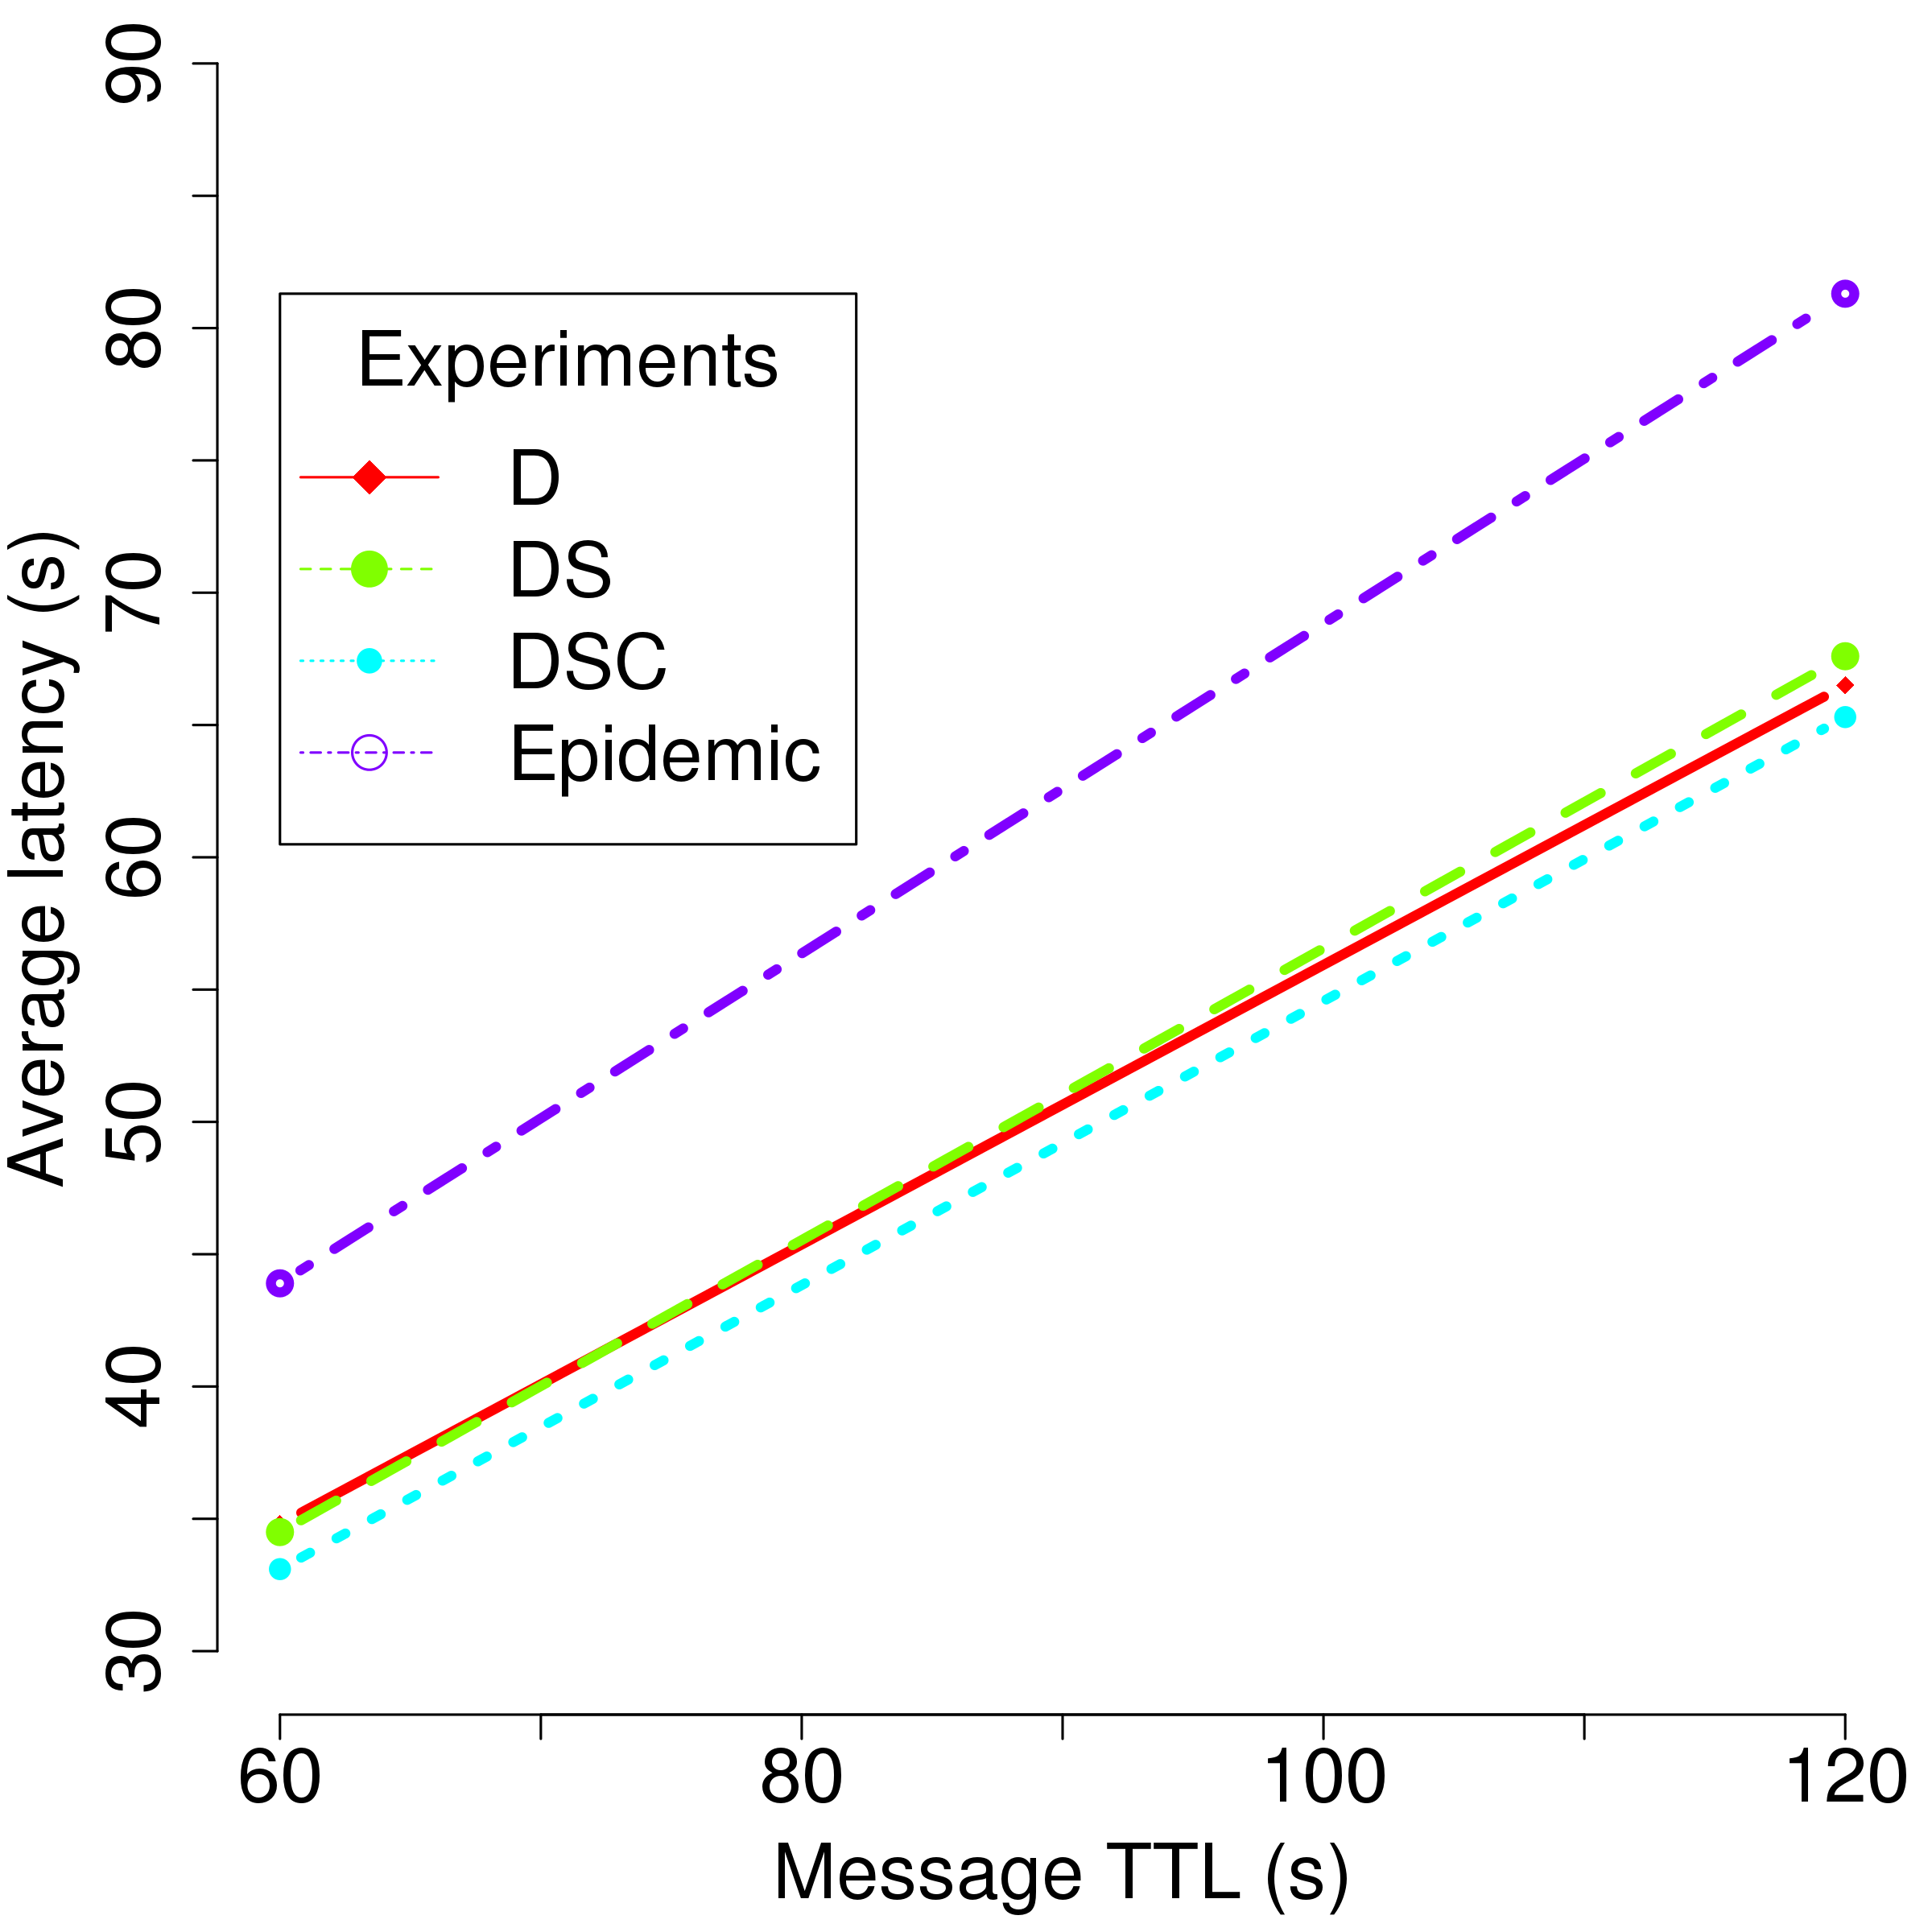
\includegraphics[width=5.3cm]{img/5.png}
        }
    }
    \caption{Average latency according to the message TTL with 30 messages} \label{grafico3}
\end{figure}

\subsection{Message packets sent}

This metric evaluates the overhead caused by the excessive creation of packets to forward the message. In both approaches (\emph{MFCV} and \emph{Epidemic}) we measured the number of message packets generated per minute, except the status beacons of both protocols. In Epidemic, we counted all the packets generated to send the \emph{summary vector} and the \emph{request messages vector} too, since they are exclusive from the protocol. As shown in the \autoref{grafico4} \emph{Epidemic} sent a massive amount of message packets per min, creating almost 800 message packets when the TTL is 60 seconds, and reaching 1000 packets when the TTL is 120 seconds. Whilst \emph{MFCV} generates relatively low amount, reaching approximately to 100 and 300 packets per minute respectively. These results demonstrate the feasibility of \emph{MFCV}.

\begin{figure}[thpb]
    \center
    \framebox{
        \parbox{2.1in}{
            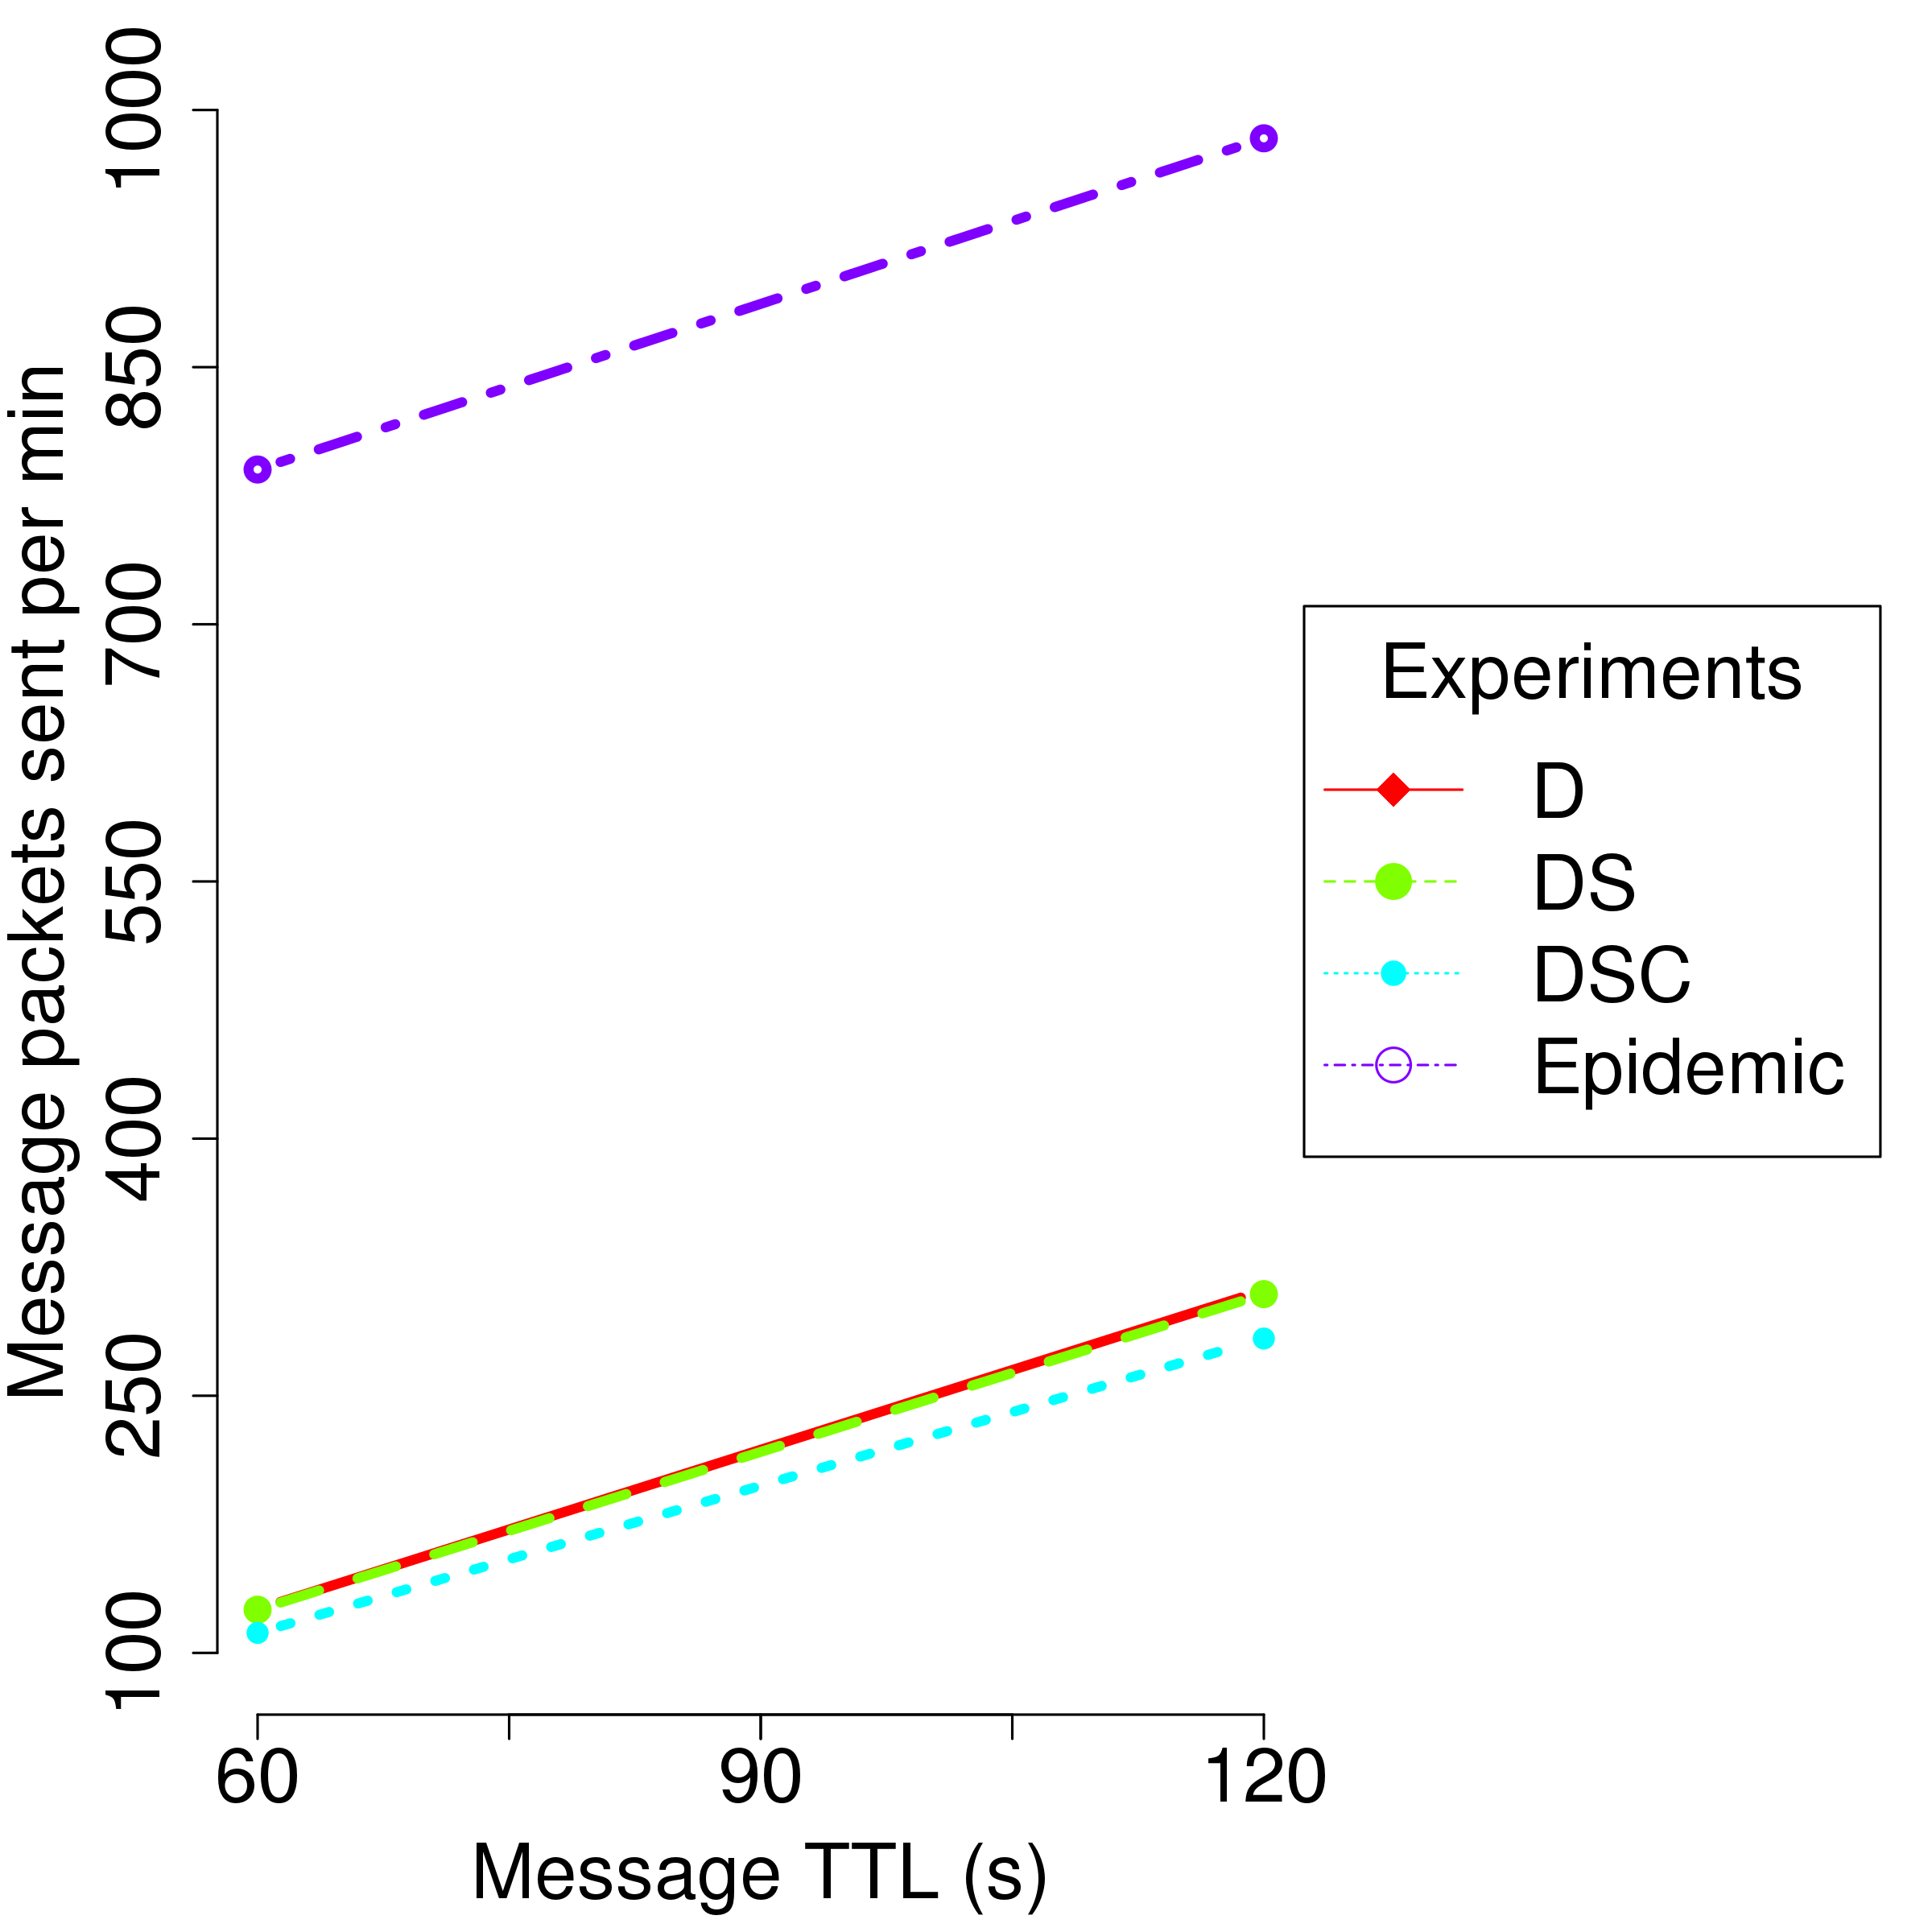
\includegraphics[width=5.3cm]{img/3.png}
        }
    }
    \caption{Message packets sent by minute on the basis of the message TTL with 30 messages} \label{grafico4}
\end{figure}

\section{CONCLUSION}

This paper presented \emph{MFCV} - a message forwarding protocol for VANETs. \emph{MFCV} exploits context information to improve the opportunistic forwarding of messages. The vehicle distance to the destination, its speed and categories (type and use), were used in the decision make to enhance the process. Vehicle usage category was used to extract mobility habits of each vehicle. We used path history of all vehicles to observe if they are approaching destination and \emph{RateTimeToSend} mechanism to control the messages forwarding rate and the number of hops. We compared our results with \emph{Epidemic} routing protocol, in terms of successful delivery rate, average latency and the number of message packets send per minute. \emph{MFCV} performed only 6 to 9\% worse than \emph{Epidemic} in terms of message delivery success. Additionally, in terms of average latency, our protocol performed 10 to 15\% better than \emph{Epidemic}. Finally, in terms of message packets sent, our protocol sent around 70\% fewer message packets, as compared with \emph{Epidemic}, in the worst case. Our results conclude that our protocol performed as good as \emph{Epidemic}. Moreover, it consumed fewer resources as well.

As a future work, we intend to evaluate the impact of buffer size, the number of messages generated and the number of vehicles using real-world mobility traces. in our forwarding scheme. Additionally, we intend to investigate other vehicles categories such as buses and trucks in different environments like city and highways. We also plan to exploit other context information such as acceleration and heading of vehicles to increase our protocol success rate in terms of message delivery and latency.

%\section*{APPENDIX}
%Appendixes should appear before the acknowledgment.

\section*{ACKNOWLEDGMENT} This research was supported by an Innovation and Dissemination Center (CEPID) grant to the Center for Research in Mathematical Sciences Applied to Industry (CeMEAI) at the University of São Paulo - FAPESP process: 2013/07375-0, and by the Coordination for the Improvement of Higher E\-du\-cation Personnel - CAPES processes PROEX-8991283/M.

\bibliographystyle{IEEEtran}

\bibliography{refs}

\end{document}
